%%%%%%%%%%%%%%%%%%%%%%%%%%%%%%%%%%%%%%%%%
% Simple Sectioned Essay Template
% LaTeX Template
%
% This template has been downloaded from:
% http://www.latextemplates.com
%
% Note:
% The \lipsum[#] commands throughout this template generate dummy text
% to fill the template out. These commands should all be removed when 
% writing essay content.
%%%%%%%%%%%%%%%%%%%%%%%%%%%%%%%%%%%%%%%%%

%----------------------------------------------------------------------------------------
%	PACKAGES AND OTHER DOCUMENT CONFIGURATIONS
%----------------------------------------------------------------------------------------

\documentclass[12pt]{book} % Default font size is 12pt, it can be changed here
		\textheight = 28cm
		\textwidth = 19cm
		\topmargin = -1cm
		\oddsidemargin = -1cm
		\parindent = 5mm

\usepackage{geometry} % Required to change the page size to A4
\geometry{a4paper} % Set the page size to be A4 as opposed to the default US Letter

\usepackage{graphicx} % Required for including pictures

\usepackage{float} % Allows putting an [H] in \begin{figure} to specify the exact location of the figure
\usepackage{wrapfig} % Allows in-line images such as the example fish picture

%\usepackage{lipsum} % Used for inserting dummy 'Lorem ipsum' text into the template

\linespread{1.1} % Line spacing

%\setlength\parindent{0pt} % Uncomment to remove all indentation from paragraphs
\usepackage[utf8]{inputenc}
\usepackage[spanish]{babel}
\usepackage[T1]{fontenc}
\usepackage{fancyhdr}

% Configurar los encabezados, pies de pagina y paginas de capitulo
% Encabezados
\lhead[\thepage]{CAPÍTULO \thechapter. \rightmark}
\chead[]{}
\rhead[CAPÍTULO \thechapter. \leftmark]{\thepage}

\renewcommand{\headrulewidth}{0.5pt}

% Pie de pagina

\lfoot[]{\today}
\cfoot[]{}
\rfoot[J.Carlos Ávila]{}
\renewcommand{\footrulewidth}{0pt}

\usepackage{savesym}
\usepackage{amsmath}
\savesymbol{iint}
\usepackage{txfonts}
\restoresymbol{TXF}{iint}


\usepackage[x11names,table]{xcolor}
\usepackage{pstricks}
\usepackage[colorinlistoftodos, textwidth=2cm, shadow]{todonotes}
%\usepackage{hyperref}



\usepackage[colorlinks]{hyperref}
\usepackage[nogroupskip,nopostdot]{glossaries}
\setglossarystyle{altlist}
\makenoidxglossaries




%\usepackage[toc,style=altlistgroup,hyperfirst=false]{glossaries}


\hypersetup{
    colorlinks=true,
    linkcolor=rosa1,
    filecolor=magenta,      
    urlcolor=cyan,
}

\urlstyle{same}

\graphicspath{{./images/}} % Specifies the directory where pictures are stored

\definecolor{miorange}{rgb}{0.11, 0.43, 0.21}
\definecolor{rosa1}{RGB}{236, 46, 80}

%%%%%%%%%%%%%%%%%%%%%%%%%%%%%%%%%%%%%%%%%%%%%%%%%%%%%%%%%%%%%%%%%%%%%%%%%%%%%%%%%%%%%%%%%%%%%%%%%%%%%%%%%%%
%----------------------------------------------------------------------------------------
%	begin {Glosario}
%----------------------------------------------------------------------------------------

\newglossaryentry{SO}{name={SO},description={Es el sistema o conjunto de aplicaciones que permiten que una computadora lleven a cabo sus funciones.}}
\newglossaryentry{Linux}{name={Linux},description={GNU/Linux Sistema Operativo creado y distribuido por miles de 
													personas alrededor del mundo}}
													
\newglossaryentry{Windows}{name={Windows},description={Sistema Operativo creado y distribuido por Microsoft.}}

\newglossaryentry{Mac}{name={Mac},description={Sistema Operativo creado y distribuido por Apple}}

%%%%%%%%%%%%%%%%%%%%%%%%%%%%%%%%%%%%%%%%%%%%%%%%  %%%%%%%%%%%%%%%%%%%%%%%%%%%%%%%%%%%%%%%%%%%%%%%%%%%%%%%%%
\newglossaryentry{}{name={},description={}}
%%%%%%%%%%%%%%%%%%%%%%%%%%%%%%%%%%%%%%%%%%%%%%%%  %%%%%%%%%%%%%%%%%%%%%%%%%%%%%%%%%%%%%%%%%%%%%%%%%%%%%%%%%

%----------------------------------------------------------------------------------------
%	End {Glosario}
%----------------------------------------------------------------------------------------


\pagestyle{fancy}

\begin{document}

\lhead[\thepage]{CAPÍTULO \thechapter. \rightmark}
\rhead[CAPÍTULO \thechapter. \leftmark]{\thepage}


%----------------------------------------------------------------------------------------
%	TITLE PAGE
%----------------------------------------------------------------------------------------

\begin{titlepage}

\newcommand{\HRule}{\rule{\linewidth}{0.5mm}} % Defines a new command for the horizontal lines, change thickness here

\center % Center everything on the page
 
%----------------------------------------------------------------------------------------
%	HEADING SECTIONS
%----------------------------------------------------------------------------------------

\textsc{\LARGE Instituto Tecnológico de San Juan del Río}\\[1.5cm] % Name of your university/college
\textsc{\Large Centro de Investigación en ciencia Aplicada y Tecnología Avanzada}\\[0.5cm] % Major heading such as course name
%\textsc{\large Minor Heading}\\[0.5cm] % Minor heading such as course title

%----------------------------------------------------------------------------------------
%	TITLE SECTION
%----------------------------------------------------------------------------------------

\HRule \\[0.4cm]
{ \huge \bfseries Amplificación interactiva de contenido por medio de la detección de la dirección de la mirada.}\\[0.4cm] % Title of your document
\HRule \\[1.5cm]
 
%----------------------------------------------------------------------------------------
%	AUTHOR SECTION
%----------------------------------------------------------------------------------------

\begin{minipage}{0.4\textwidth}
\begin{flushleft} \large
\emph{Autor:}\\
J. Carlos \textsc{\'Avila Resendiz} % Your name
\end{flushleft}
\end{minipage}
~
\begin{minipage}{0.4\textwidth}
\begin{flushright} \large
\emph{Supervisor:} \\
Dr. Joaquin  \textsc{Salas Rodriguez} % Supervisor's Name
\end{flushright}
\end{minipage}\\[4cm]

% If you don't want a supervisor, uncomment the two lines below and remove the section above
%\Large \emph{Author:}\\
%John \textsc{Smith}\\[3cm] % Your name


%----------------------------------------------------------------------------------------
%	DATE SECTION
%----------------------------------------------------------------------------------------

{\large \today}\\[1cm] % Date, change the \today to a set date if you want to be precise

%----------------------------------------------------------------------------------------
%	LOGO SECTION
%----------------------------------------------------------------------------------------


\includegraphics{./imagenes/itsjr_s.jpg}\\ % Include a department/university logo - this will require the graphicx package

 
%----------------------------------------------------------------------------------------

\vfill % Fill the rest of the page with whitespace
\newpage
$\ $
\thispagestyle{empty}
\end{titlepage}

%----------------------------------------------------------------------------------------
%	TABLE OF CONTENTS
%----------------------------------------------------------------------------------------j
\setcounter{tocdepth}{3}   %control deptness index
%\setcounter{lofdepth}{2}  % control table of figures depth 
\pagenumbering{roman} 
\tableofcontents % Include a table of contents

\newpage % Begins the essay on a new page instead of on the same page as the table of contents
\thispagestyle{empty} 
%\appendix
%----------------------------------------------------------------------------------------
%	INTRODUCTION
%----------------------------------------------------------------------------------------
\pagenumbering{arabic}	
%\setcounter{page}{1}
	
			 
\newpage		 
\pagestyle{fancy}


\chapter{GENERALIDADES}
\thispagestyle{empty}
\markboth{GENERALIDADES}{GENERALIDADES}

\begin{minipage}{0.5\textwidth}
	\begin{flushleft} \large
	%\emph{•} \\
	\scriptsize	\textsl{\large “El auténtico genio consiste en la capacidad para evaluar información incierta, 
								aleatoria y contradictoria.”}\\
	\scriptsize \textbf{Winston Churchill, estadista.}
	\end{flushleft}
\end{minipage}\\[4cm]			

\newpage
\section{Objetivos}
	\subsection{Objetivo general}
	
		Desarrollar una aplicación de amplificación interactiva para computadoras con sistema operativo Windows, 
		que asista a personas con bajas capacidades visuales, por medio del seguimiento y estimación de la dirección 
		de la mirada sobre la pantalla de la computadora y en base a ello amplificar la zona de la pantalla en la 
		que enfoca la vista.
	
	\subsection{Objetivos específicos}
		\begin{itemize}
			\item Detección precisa y confiable del movimiento del globo ocular, con la ayuda de software de 
			procesamiento de imágenes digitales.
			\item Hacer uso de las API’s del sistema operativo que proveen las herramientas que magnifican la zona de
			la pantalla seleccionada.
			\item Integrar los dos componentes anteriores y de esa forma obtener un magnificador con interacción visual.
			\item Una vez se cuente con un prototipo, realizar pruebas de campo.
		\end{itemize}
		

\newpage
\section{Justificación}
	Pese al avance desmesurado de la tecnología en los últimos años en donde las capacidades de los dispositivos se
	duplica cada cierto tiempo, respondiendo de forma bastante precisa la emblemática ley de 
	\href{https://en.wikipedia.org/wiki/Moore's_law}{Moore} hay aun a día de hoy
	ciertas cuestiones que no han sido abordadas, quizá en gran parte debido al amplio panorama de problemas que se
	pueden afrontar con soluciones tecnológicas y de alguna forma ayudar a solventar o/y hacer más fácil las mismas.
	
	Aun si los programas de asistencia a personas con capacidades diferentes están a día de hoy cobrando mayor 			  	
	relevancia en prácticamente todos los aspectos sociales, pues en la actualidad las posibilidades de llevar una vida
	productiva y sin las limitaciones de antaño, son ya una realidad, entre las herramientas que se proporcionan a este
	sector de la población están las llamadas tecnologías de asistencia o accesibilidad en entornos informáticos, mismas
	que van desde iconos monocromáticos de un mayor tamaño, hasta lectores de pantalla y lupas, siendo estas últimas el
	principal componente proporcionado por las herramientas de accesibilidad de los Sistemas Operativos \gls{SO} actuales,
	siendo común en los tres mas importantes \gls{Linux}, \gls{Windows}, \gls{Mac}.
	
	Siendo de los tres el segundo, Windows, en el cual se enfocaran los esfuerzos de hacer converger las herramientas de
	accesibilidad ya mencionadas y las tecnologías de visión por computadora CV, para ofrecer a los discapacitados 
	visuales una forma de hacer uso de la tecnología, mismos que según datos de la OMS de 2002, eran mas de 161 millones
	de personas, en especifico de computadoras, sin que su limitante visual les impida el poder interactuar con el 
	equipo.
	
	Específicamente el segmento de la población con discapacidad visual en el que se enfoca el desarrollo de este
	proyecto es el de personas que cuentan con cierto grado de visión, o lo que se conoce como resto visual, pues,
	siempre que exista un resto visual por mínimo que sea se debe potenciar su uso para alcanzar el máximo desarrollo
	posible

\newpage 
\section{Caracterización de la empresa}
	\subsection{Datos generales de la empresa}
	\begin{description}
		\item[Nombre de la organización:] Centro de Investigación en Ciencia Aplicada y Tecnología Avanzada del
			 Instituto Politécnico Nacional \texttt{CICATA}
			 
		\item[Dirección:] Querétaro, Cerro Blanco No.141 Col. Colinas del Cimatario, C.P. 76090, Querétaro, Querétaro
			 México.
			 \begin{center}
			 	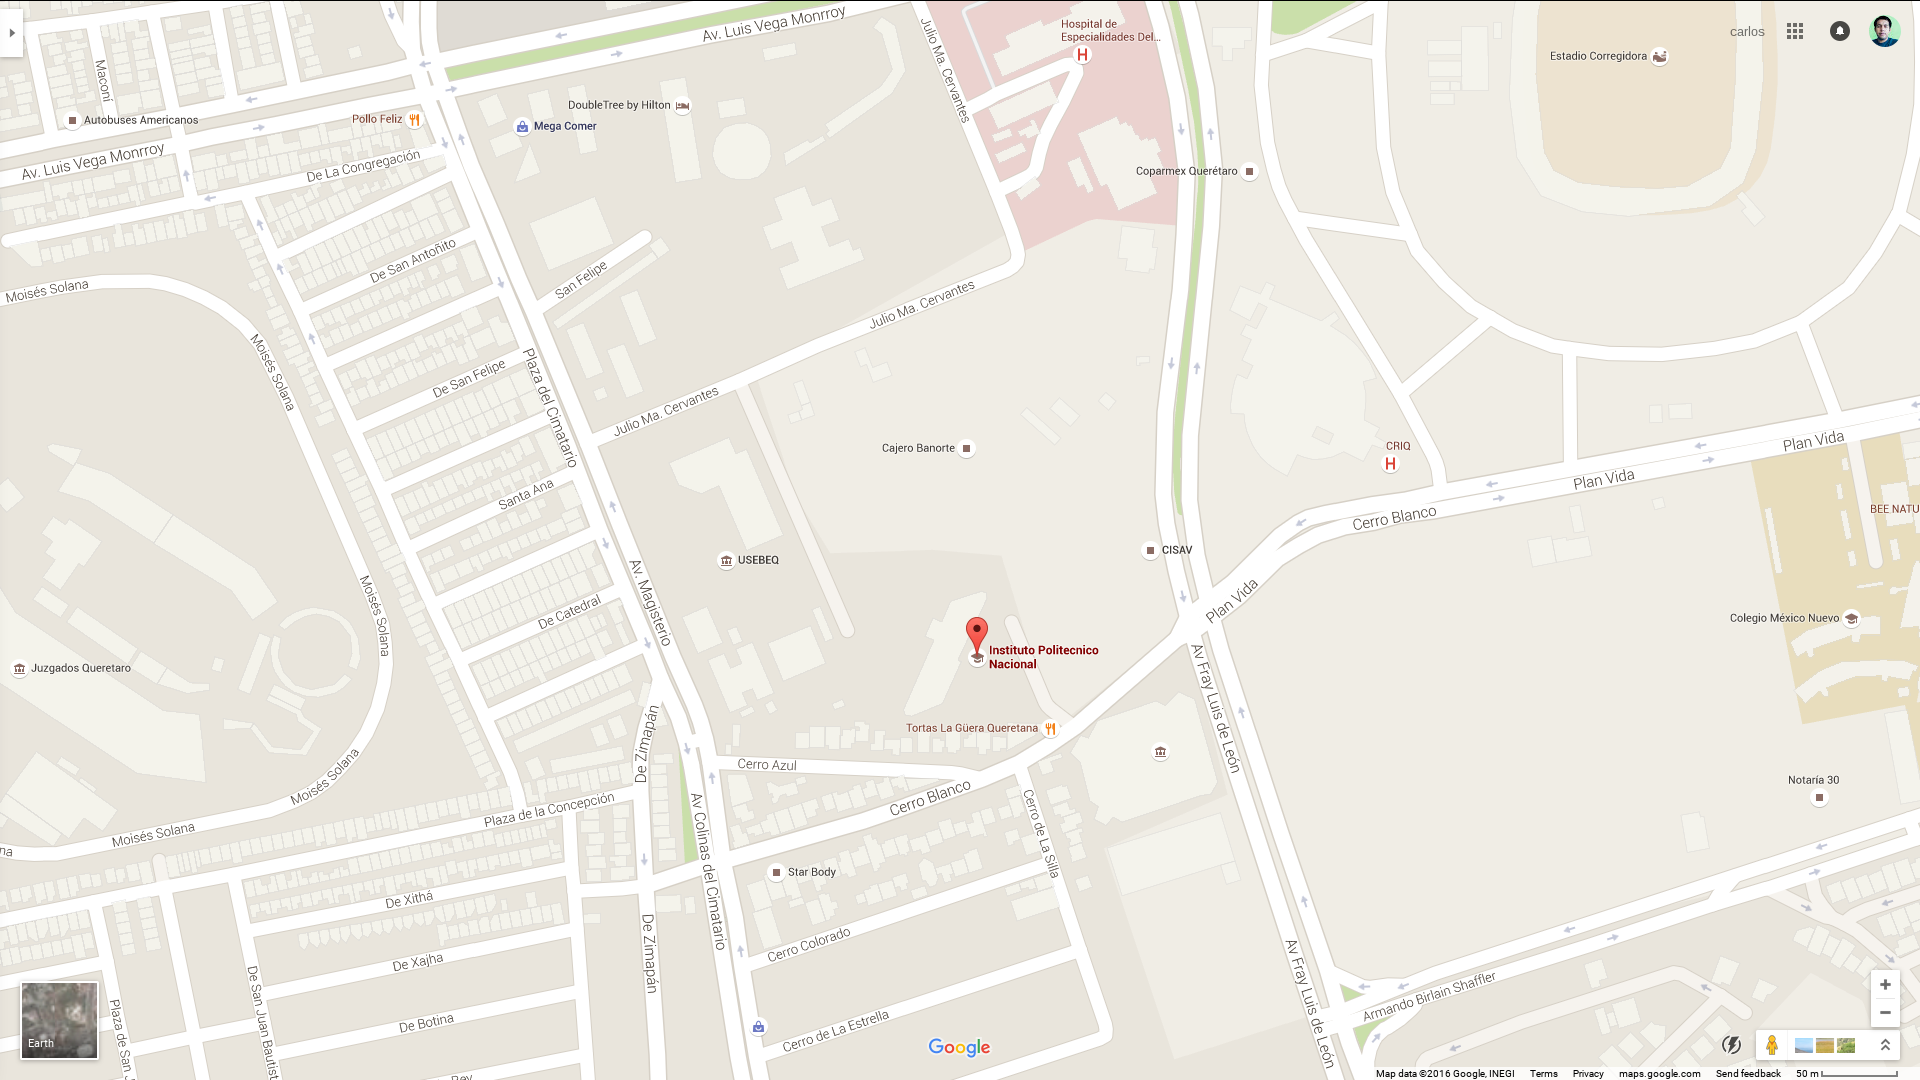
\includegraphics[width=0.9\textwidth]{./imagenes/cicata}
			 \end{center}
		\item[Teléfonos:] 1 (442) 2290804 o 01 (55) 5729 6000 Ext. 81002
		\item[E-Mail:] cicata@ipn.mx 
		\item[Fax:] 5395 4147
	\end{description}
		\subsubsection{Misión}
			Somos un centro de investigación creado por el IPN para fortalecer su impacto a nivel nacional, que atiende
			necesidades de formación de recursos humanos y de desarrollo tecnológico de la región, a través de proyectos
			de investigación que contribuyen al desarrollo social y a la competitividad de los sectores productivo y de
			servicios, con el respaldo de las capacidades del Instituto, con un enfoque multidisciplinario, innovador y
			de excelencia, en un marco de sustentabilidad.
		
		\subsubsection{Visión}
			En el 2025, el CICATA-Querétaro se ve como un centro de vanguardia en la investigación y formación de 
			recursos humanos; referente a nivel latinoamericano; con reconocimiento internacional por sus contribuciones
			de alto impacto y como una de las primeras opciones para alumnos e investigadores, por ser un centro
			innovador, competitivo, líder y emprendedor.
		
		\subsubsection{Valores}
			Hemos identificado un conjunto de valores que nos representan y que permiten cumplir nuestra misión y lograr
			la visión forjada:
			
			\begin{itemize}
				\item Calidad
				\item Integridad
				\item Compromiso
				\item Asertividad
				\item Trabajo en equipo
				\item Aprendizaje continuo
			\end{itemize}
		
		\subsubsection{Objetivo}
			Servir de enlace entre la comunidad científica y los sectores productivos de bienes y servicios, atenderlos
			y ofrecerles soluciones a sus problemas de desarrollo. Para el cumplimiento de este objetivo, CICATA
			Querétaro desarrolla programas de investigación científica, tecnológica e innovación con un enfoque
			interdisciplinario, y asimismo atiende la formación de capital humano de alto nivel, contribuyendo
 			decisivamente al fortalecimiento de la calidad y la competitividad del aparato productivo mexicano.
 		
 		\subsubsection{Estructura Organizativa}
 			\begin{center}
			 	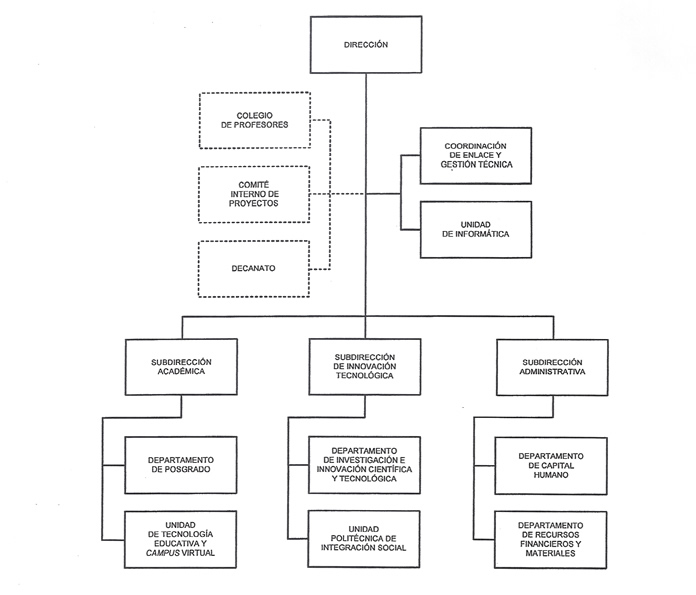
\includegraphics[width=0.9\textwidth]{./imagenes/organigrama}
			 \end{center}
			 
	
	\subsection{Descripción del departamento o área de trabajo}
		 El área de análisis de imágenes puede ser definida como la construcción de algoritmos para la extracción de 
		 información presente en las imágenes. Es un área donde una gran variedad de conceptos fundamentales necesitan 
		 ser desarrollado e importantes aplicaciones pueden crearse. Esta combinación de teoría y práctica es particularmente 
		 atractiva para CICATA Querétaro en virtud de corresponder con su objetivo operativo. El grupo de análisis de imágenes 
		 ha presentado desde sus orígenes resultados muy buenos en el renglón de vinculación y desarrollo tecnológico.  
		 Se han trabajado proyectos de vinculación con empresas e instituciones tales como TAMSA y el IFE, por mencionar algunos. 
		 En la actualidad con un grupo de cuatro investigadores esta tendencia se ha mantenido.  En este momento se estudian 
		 temas de interferometría, colorimetría, industrial, metrología, óptica, análisis de imágenes, procesamiento de imágenes, 
		 reconstrucción tridimensional e interpretación visual de la actividad.

\newpage
\section{Problemas a resolver}
	\begin{itemize}
		\item 
	\end{itemize}
\newpage
\section{Alcances y limitaciones}
	\subsection{Alcances}
	\subsection{Limitaciones}




\chapter{FUNDAMENTACIÓN TEÓRICA}
\markboth{FUNDAMENTACIÓN TEÓRICA}{FUNDAMENTACIÓN TEÓRICA} 
\thispagestyle{empty}

\section{Ingeniería del software}

\section{Herramientas de desarrollo}
	
	\subsection{Visual Studio Community 2015}
		\textsc{Visual Studio Community 2015} es un entorno de desarrollo integrado creado y distribuido por \textsc{Microsoft}, 
		para el sistema operativo de la misma.
		Soporta una gran variedad de lenguajes de programación tales como, \textsc{ C++, C\#, Visual Basic, .NET, F\#, Java, Python, 
		Ruby, PHP}, al igual que entornos de desarrollo web como \textsc{ASP.NET MVC, Django, etc.,} a lo cual sumarle las nuevas
		capacidades online bajo Windows Azure en forma del editor Monaco.
		Esta version en particular tiene la particularidad de ser gratuita e incluir todas las características de la versión 
		\textsc{Express}, enfocada en desarrolladores individuales, proyectos de código abierto, investigación académica, educación
		y pequeños equipos profesionales.
		
	\subsection{MariaDB}
		\textsc{MariaDB} es un sistema de gestión de bases de datos derivado de \textsc{MySQL} con licencia \textsc{GPL}. 
		Está desarrollado por \textit{Michael (Monty) Widenius (fundador de MySQL)} y la comunidad de desarrolladores de software 
		libre. 
		
		Introduce dos motores de almacenamiento nuevos, uno llamado Aria -que reemplaza con ventajas a \textsc{MyISAM}- y otro
		lamado \textsc{XtraDB} -en sustitución de \textsc{InnoDB}. Tiene una alta compatibilidad con MySQL ya que posee las mismas
		órdenes, interfaces, APIs y bibliotecas, siendo su objetivo poder cambiar un servidor por otro directamente. 
		Este \textsc{SGBD} surge a raíz de la compra de \textit{Sun Microsystems}.
		
		MariaDB es un fork directo de MySQL que asegura que permanecerá una versión de este producto con licencia GPL.
		
	\subsection{SQLite}
		\textsc{SQLite} es un sistema de gestión de bases de datos relacional compatible con \textsc{ACID}, contenida en una
		relativamente pequeña (~275 kiB) biblioteca escrita en C. SQLite es un proyecto de dominio público creado por 
		\textit{D. Richard Hipp}.
		
		A diferencia de los sistema de gestión de bases de datos cliente-servidor, el motor de SQLite no es un proceso independiente 
		con el que el programa principal se comunica. En lugar de eso, la biblioteca SQLite se enlaza con el programa pasando a ser
		parte integral del mismo. 
		
		El programa utiliza la funcionalidad de SQLite a través de llamadas simples a subrutinas y funciones. Esto reduce la latencia 
		en el acceso a la base de datos, debido a que las llamadas a funciones son más eficientes que la comunicación entre procesos. 
		El conjunto de la base de datos (definiciones, tablas, índices, y los propios datos), son guardados como un sólo fichero
		estándar en la máquina cliente. 
		Este diseño simple se logra bloqueando todo el fichero de base de datos al principio de cada transacción.
		
		En su versión 3, SQLite permite bases de datos de hasta \textsc{2 Terabytes} de tamaño, y también permite la inclusión de campos
		tipo \textsc{BLOB}.
		
	\subsection{IntraFace}
		IntraFace es una librería que incluye algoritmos para análisis de patrones faciales, se comenzó a desarrollar en 2010 en la
		universidad \textsc{Carnigie Mellon y University of Pittsburgh}, actualmente la ultima version de la misma es la 1.0, soportada 
		por Human Sensing Laboratory.
		Para este proyecto se usa una version anterior de la misma, provista para fines educativos y/o investigación sin fines de lucro.

	\subsection{OpenCV}
		\textsc{OpenCV} es una biblioteca libre de visión artificial originalmente desarrollada por \textbf{Intel}. 
		Desde que apareció su primera versión alfa en el mes de enero de 1999, se ha utilizado en infinidad de aplicaciones. 
		Desde sistemas de seguridad con detección de movimiento, hasta aplicaciones de control de procesos donde se requiere
		reconocimiento de objetos. Esto se debe a que su publicación se da bajo licencia \textsc{BSD}, que permite que sea usada
		libremente para propósitos comerciales y de investigación con las condiciones en ella expresadas.
		
		OpenCV es multiplataforma, existiendo versiones para \textsc{GNU/Linux, Mac OS X y Windows}. Contiene más de 500 funciones 
		que abarcan una gran gama de áreas en el proceso de visión, como reconocimiento de objetos (reconocimiento facial), 
		calibración de cámaras, visión estérea y visión robótica.
		
		El proyecto pretende proporcionar un entorno de desarrollo fácil de utilizar y altamente eficiente. Esto se ha logrado
		realizando su programación en código C y C++ optimizados, aprovechando además las capacidades que proveen los procesadores
		multinúcleo. OpenCV puede además utilizar el sistema de primitivas de rendimiento integradas de Intel, un conjunto de 
		rutinas de bajo nivel específicas para procesadores Intel \textsc{(IPP)}.
		
	
\section{Lenguajes de programación}
	Un lenguaje de programación es una herramienta que nos permite comunicarnos e instruir a la computadora para que realice una tarea
	especifica. Cada lenguaje de programacion posee una sintaxis y un léxico particular, es decir, la forma de escribirse, que es 
	diferente en cada uno por la forma en que fue creado y por la forma que trabaja su compilador para revisar, acomodar y reservar el
	programa en memoria.
	
	Existen muchos lenguajes, sin embargo en este proyecto solo nos interesan los siguientes:
	\begin{itemize}
		\item C++
		\item Python
		\item R		
	\end{itemize}

	\subsection{C++}
		\textsc{C++} es un lenguaje de programación diseñado a mediados de los años 1980 por \textit{Bjarne Stroustrup}. La intención 
		de su creación fue el extender al lenguaje de programación \textsc{C}, agregando mecanismos que permitieran la manipulación de
		objetos. En ese sentido, desde el punto de vista de los lenguajes orientados a objetos, el C++ es un lenguaje híbrido.
		
		Posteriormente se añadieron facilidades de programación genérica, que se sumaron a los paradigmas de programación estructurada 
		y programación orientada a objetos. Por esto se suele decir que el C++ es un lenguaje de programación multiparadigma.

		Actualmente existe un estándar, denominado \textsc{ISO C++,} al que se han adherido la mayoría de los fabricantes de 
		compiladores más modernos. Existen también algunos intérpretes, tales como ROOT.
	
	\subsection{Python}
	
	\subsection{R}
		
\newpage
\section{Metodologías de desarrollo de software}


\chapter{DESCRIPCIÓN DE ACTIVIDADES REALIZADAS}
\markboth{ACTIVIDADES REALIZADAS}{ACTIVIDADES REALIZADAS}
\thispagestyle{empty}
\newpage
\section{Análisis}

\section{Diseño}

\section{Desarrollo}

\section{Pruebas}

\section{Implementación}

\section{Retroalimentación}

\section{Resultados}

\section{Conclusiones y recomendaciones}

\section{Referencias Bibliográficas \& Glosario} 	
%----------------------------------------------------------------------------------------
%	BEGIN GLOSARIO
%----------------------------------------------------------------------------------------			
\newpage


\printnoidxglossaries
\pagenumbering{roman}

%----------------------------------------------------------------------------------------
%	END GLOSARIO
%----------------------------------------------------------------------------------------


%---------------------------------------------------------------------------------------
%	BIBLIOGRAPHY
%----------------------------------------------------------------------------------------

\begin{thebibliography}{99} % Bibliography - this is intentionally simple in this template




%\bibitem{Luckham} 
%David Luckham
%[\textit{The Power of Events - An Introduction to Complex Event Processing in Distributed Enterprise Systems}]. 
%Addison-Wesley, ISBN 0-201-72789-7.


%\bibitem{Tello} 
%Adolfo Lozano Tello
%[\textit{Iniciación a la programación utilizando lenguajes visuales orientados a eventos.}] [ISBN978-84-7897-714-7]
%Ed.Bellisco Ediciones Técnicas y Científicas, ISBN 84-95279-49-5. ISBN 978-84-95279-49-1.


%\bibitem{} 
%Ricardo Barona Vázquez
%[\textit{Asterisk©, telefonía IP en software libre}].
%\href{Asterisk}{ http://www.enterate.unam.mx/artic/2008/abril/art3.html}

\end{thebibliography}


%----------------------------------------------------------------------------------------
 
\end{document}


